\documentclass{article}

\usepackage{fullpage}
\usepackage{pdfpages}
\usepackage{hyperref}
\usepackage{titlesec}

\hypersetup{
    colorlinks,
    citecolor=black,
    filecolor=black,
    linkcolor=blue,
    urlcolor=black,
    	linktoc=all
}

\pagestyle{empty}

\newcommand{\GradedWork}[2]{%
\phantomsection
\addtocounter{subsection}{1}
\addcontentsline{toc}{subsection}{#1}
\includepdf[pages={-},addtotoc={1,subsubsection,2,#1 - Best,assign:#2-best}]{graded/#2-best.pdf}
\includepdf[pages={-},addtotoc={1,subsubsection,2,#1 - Average,assign:#2-average}]{graded/#2-average.pdf}
\includepdf[pages={-},addtotoc={1,subsubsection,2,#1 - Worst,assign:#2-worst}]{graded/#2-worst.pdf}
}%

\begin{document}

\newpage
\tableofcontents

\vspace{0.5in}


\titleformat{\section}
	{\LARGE\bfseries\centering}{}{1em}{\vfill}[\vfill]

\newpage

\section{Syllabus}
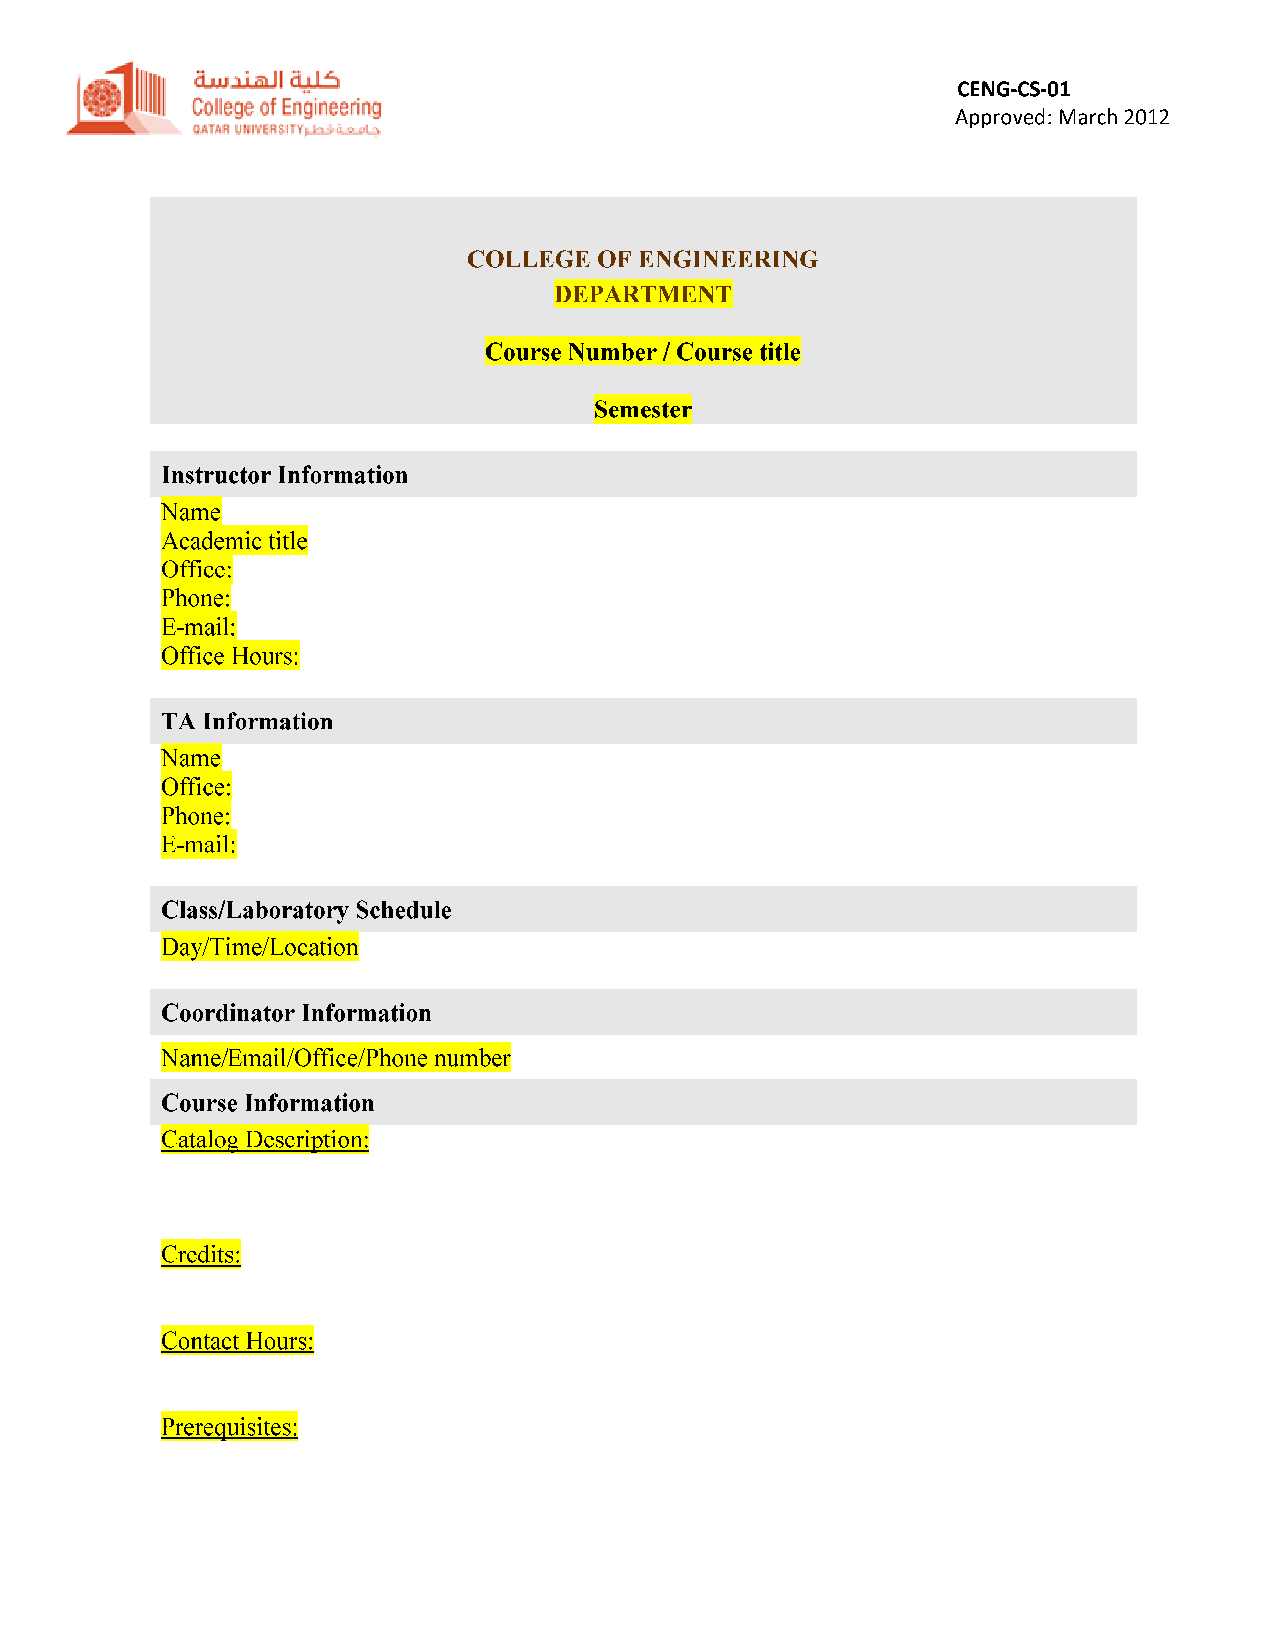
\includepdf[pages={-},addtotoc={1,subsection,2,Unified College Syllabus,syl:col}]{syllabus/syllabus.pdf}

\newpage
\section{Copies of Assignments}
\newpage


\includepdf[pages={-},addtotoc={1,subsection,2,Homework 1,assign:hw1}]{coursework/hw1.pdf}


\includepdf[pages={-},addtotoc={1,subsection,2,Homework 2,assign:hw2}]{coursework/hw2.pdf}


\includepdf[pages={-},addtotoc={1,subsection,2,Midterm Exam,assign:midterm}]{coursework/midterm.pdf}


\includepdf[pages={-},addtotoc={1,subsection,2,Final Exam,assign:final}]{coursework/final.pdf}

\newpage
\section{Student Performance/Grades}

\includepdf[pages={-}]{other/grades.pdf}

\end{document}